% ============================================================================
% Template Jurnal Penulisan Ilmiah - Teknik Informatika
% Universitas Gunadarma
%
% Judul: Deteksi Area Infeksi Pneumonia pada Citra Rontgen Dada
%        Menggunakan Arsitektur U-Net dan Atensi sCSE
% ============================================================================
\documentclass[12pt,a4paper,twocolumn]{article}

% --- Packages ---------------------------------------------------------------
\usepackage[T1]{fontenc}
\usepackage[utf8]{inputenc}
\usepackage[indonesian]{babel}       % Bahasa Indonesia support
\usepackage{mathptmx}                % Times New Roman font
\usepackage{geometry}                % Page margins
\usepackage{setspace}                % Line spacing
\usepackage{graphicx}                % Images
\usepackage{amsmath,amssymb}         % Mathematical equations
\usepackage{caption}                 % Caption formatting
\usepackage{natbib}                  % Author-date citation style
\usepackage{url}                     % URL formatting
\usepackage{booktabs}                % Professional tables
\usepackage{array}                   % Extended table columns
\usepackage{titlesec}                % Section title formatting
\usepackage{fancyhdr}                % Headers and footers
\usepackage{abstract}                % Abstract formatting
\usepackage{indentfirst}             % Indent first paragraph of sections
\usepackage{listings}                % Code listings
\usepackage{xcolor}                  % Color support for listings
\usepackage{tabularx}                % Flexible-width tables
\usepackage{multirow}                % Multi-row cells in tables
\usepackage{float}                   % Force float placement with [H]
\usepackage{hyperref}                % Hyperlinks (load last)

% --- Path Gambar & Compat Macros --------------------------------------------
\graphicspath{{../img/}{gambar/}}
\newcommand{\parencite}[1]{\citep{#1}}
\newcommand{\textcite}[1]{\citet{#1}}

% --- Listings Setup ---------------------------------------------------------
\lstset{
    basicstyle       = \ttfamily\scriptsize,
    keywordstyle     = \color{blue}\bfseries,
    commentstyle     = \color{gray},
    stringstyle      = \color{red},
    breaklines       = true,
    frame            = single,
    numbers          = none,
    showstringspaces = false,
    tabsize          = 2,
    captionpos       = b
}

% --- Page Layout ------------------------------------------------------------
\geometry{
    a4paper,
    left   = 3cm,
    right  = 3cm,
    top    = 3cm,
    bottom = 3cm
}

% --- Spacing ----------------------------------------------------------------
\onehalfspacing                      % 1.5 line spacing
\setlength{\columnsep}{1cm}          % Column separation

% --- Section Formatting -----------------------------------------------------
% Sections: uppercase, bold, centered, 12pt
\titleformat{\section}
    {\normalfont\normalsize\bfseries\MakeUppercase}
    {}
    {0pt}
    {}
\titlespacing*{\section}{0pt}{12pt}{6pt}

% Subsections: bold, left-aligned, 12pt
\titleformat{\subsection}
    {\normalfont\normalsize\bfseries}
    {}
    {0pt}
    {}
\titlespacing*{\subsection}{0pt}{10pt}{4pt}

% Remove section numbering as per journal format
\setcounter{secnumdepth}{0}

% --- Caption Formatting -----------------------------------------------------
\captionsetup{
    font       = {small},            % 10pt caption text
    labelfont  = {bf},               % Bold "Tabel 1." / "Gambar 1."
    labelsep   = period,             % Period after number
    justification = centering,
    singlelinecheck = false
}
\captionsetup[table]{position = above}
\captionsetup[figure]{position = below}

% --- Citation Style ---------------------------------------------------------
\bibliographystyle{apalike}          % Author-date style

% --- Hyperlink Setup --------------------------------------------------------
\hypersetup{
    colorlinks  = true,
    linkcolor   = black,
    citecolor   = black,
    urlcolor    = blue
}

% ============================================================================
% DOCUMENT START
% ============================================================================
\begin{document}

% --- Title ------------------------------------------------------------------
\twocolumn[
\begin{@twocolumnfalse}
\begin{center}

% JUDUL
{\bfseries DETEKSI AREA INFEKSI PNEUMONIA PADA CITRA RONTGEN DADA \\
MENGGUNAKAN ARSITEKTUR U-NET DAN ATENSI sCSE}

\vspace{12pt}

% AUTHORS
{\normalsize
Muhammad Hisyam\textsuperscript{1} Dr. Tavipia Rumambi, SKom., MMSI.\textsuperscript{2}
}

\vspace{8pt}

% AFFILIATIONS
{\small
\textsuperscript{1}Fakultas Teknologi Industri, Universitas Gunadarma \textsuperscript{2}Fakultas Teknologi Industri, Universitas Gunadarma \\
Jl. Margonda Raya No. 100, Depok 16424, Jawa Barat \\[4pt]
\textsuperscript{1}\texttt{51422075@student.gunadarma.ac.id}, \textsuperscript{2}\texttt{tavipia@staff.gunadarma.ac.id}
}

\vspace{16pt}

% % --- ABSTRAK (Bahasa Indonesia) --------------------------------------------
\begin{minipage}{0.85\textwidth}
\begin{center}
    {\normalsize\bfseries ABSTRAK}
\end{center}
\vspace{-14pt}
{\footnotesize\itshape\singlespacing
Tingginya angka kematian akibat pneumonia pada anak-anak, lansia, dan pasien dengan imunitas rendah di seluruh dunia, ditambah keterbatasan interpretasi citra radiografi dada (\textit{Chest X-Ray}/CXR) secara manual yang memerlukan keahlian khusus dan waktu yang tidak sedikit, mendorong kebutuhan sistem deteksi otomatis berbasis \textit{deep learning}. Penelitian ini membangun sistem deteksi dan segmentasi area infeksi pneumonia secara otomatis pada citra CXR dengan pendekatan \textit{deep learning} mengikuti kerangka \textit{CRISP-DM}. Pendekatan \textit{dual masking} diterapkan, di mana masker paru-paru yang dihasilkan secara otomatis oleh model PSPNet digunakan untuk membatasi wilayah analisis, sementara masker anotasi pneumonia digunakan sebagai \textit{ground truth} latih. Segmentasi dilakukan menggunakan arsitektur \textbf{U-Net dengan mekanisme atensi sCSE} (\textit{Spatial and Channel Squeeze-and-Excitation}) dan \textit{backbone} \textbf{EfficientNet-B3} \textit{pretrained} ImageNet, yang dilatih pada dataset \textit{RSNA Pneumonia Detection Challenge} (26.684 citra) menggunakan fungsi kerugian \textbf{\textit{Unified Focal Loss}}, optimizer AdamW, serta \textit{Automatic Mixed Precision} dengan akumulasi gradien. Keterjelasan keputusan model difasilitasi menggunakan \textbf{Grad-CAM}, dan sistem diintegrasikan ke dalam antarmuka web interaktif berbasis \textbf{Gradio} yang dapat diakses melalui internet menggunakan \textbf{Cloudflare Tunnel}. Hasil evaluasi kuantitatif menunjukkan kinerja tinggi dengan \textit{Dice Coefficient} sebesar \textbf{0,6234}, \textit{Precision} sebesar \textbf{0,6868}, \textit{Recall} sebesar \textbf{0,7082}, dan \textit{Specificity} sebesar \textbf{0,9781}, membuktikan bahwa sistem ini berpotensi menjadi alat bantu skrining awal yang efektif dan transparan untuk tenaga medis.
\par}

\vspace{6pt}
{\footnotesize\textbf{Kata Kunci:} \textit{Deep Learning, EfficientNet-B3, Pneumonia, sCSE, U-Net.}}
\end{minipage}

\vspace{16pt}

% --- ABSTRACT (English) ----------------------------------------------------
\begin{minipage}{0.85\textwidth}
\begin{center}
    {\normalsize\bfseries ABSTRACT}
\end{center}
\vspace{-14pt}
{\footnotesize\itshape\singlespacing
The high mortality rate caused by pneumonia among children, the elderly, and immunocompromised patients worldwide, combined with the limitations of manual chest X-ray (CXR) interpretation that requires specialized expertise and considerable time, drives the need for an automated deep learning-based detection system. This study builds an automated pneumonia infection area detection and segmentation system on CXR images using a deep learning approach following the CRISP-DM framework. A dual-masking strategy is applied, where an automatically generated lung segmentation mask from the PSPNet model constrains the analysis region, while an annotated pneumonia mask serves as the training ground truth. Segmentation is performed using the \textbf{U-Net architecture with sCSE attention} (\textit{Spatial and Channel Squeeze-and-Excitation}) and a \textbf{pretrained EfficientNet-B3 backbone} (ImageNet), trained on the \textit{RSNA Pneumonia Detection Challenge} dataset (26,684 images) with the \textbf{Unified Focal Loss} function, AdamW optimizer, and Automatic Mixed Precision with gradient accumulation. Model decision explainability is provided by \textbf{Grad-CAM}, and the system is integrated into an interactive web interface built on \textbf{Gradio}, accessible over the internet via \textbf{Cloudflare Tunnel}. Quantitative evaluation results demonstrate high segmentation performance with a \textit{Dice Coefficient} of \textbf{0.6234}, \textit{Precision} of \textbf{0.6868}, \textit{Recall} of \textbf{0.7082}, and \textit{Specificity} of \textbf{0.9781}, confirming the system's potential as an effective and transparent early screening tool for medical personnel.
\par}

\vspace{6pt}
{\footnotesize\textbf{Keywords:} \textit{Deep Learning, EfficientNet-B3, Pneumonia, sCSE, U-Net.}}
\end{minipage}

\vspace{20pt}

\end{center}
\end{@twocolumnfalse}
]

% ============================================================================
% PENDAHULUAN
% ============================================================================
\section{Pendahuluan}

Tingginya angka morbiditas dan mortalitas akibat infeksi pernapasan akut menempatkan kondisi ini sebagai salah satu ancaman kesehatan utama di tingkat global maupun nasional. Berdasarkan data \textit{World Health Organization} (WHO), infeksi ini merenggut sekitar 2,5 juta jiwa di seluruh dunia pada tahun 2019, dengan porsi terbesar menyerang kelompok rentan seperti anak-anak di bawah usia lima tahun \parencite{who2022}. Di Indonesia, beban penyakit ini sangat signifikan dan diperparah oleh keterbatasan sarana penunjang diagnosis medis di daerah perifer \parencite{said2018}. Secara klinis, patologi ini terjadi saat patogen seperti bakteri, virus, atau jamur menginvasi paru-paru dan memicu penumpukan cairan eksudat pada kantung udara (\textit{alveoli}), yang berujung pada kegagalan fungsi ventilasi paru-paru dan sesak napas akut \parencite{seth2022}.

Cara yang paling umum digunakan untuk mendiagnosis pneumonia adalah melalui pemeriksaan foto rontgen dada (\textit{Chest X-Ray}/CXR). Pemeriksaan ini dipilih karena biayanya terjangkau, mudah didapat, dan dosis radiasinya lebih rendah dibandingkan CT Scan. Namun, membaca foto rontgen secara manual memiliki beberapa kelemahan. Radiolog yang kelebihan beban kerja dapat memperlambat proses diagnosis. Selain itu, pola infeksi pneumonia pada foto rontgen kadang mirip dengan penyakit paru lain seperti edema atau efusi pleura, sehingga rawan salah baca --- terutama di fasilitas yang kekurangan tenaga ahli. Oleh karena itu, dibutuhkan sistem yang dapat membantu dokter mendeteksi pneumonia secara otomatis agar diagnosis bisa lebih cepat dan konsisten.

Dalam beberapa tahun terakhir, teknologi \textit{deep learning} berbasis \textit{Convolutional Neural Network} (CNN) terbukti mampu menganalisis citra medis dengan tingkat akurasi yang tinggi. Salah satu arsitektur yang banyak digunakan untuk analisis citra medis adalah U-Net, yang diperkenalkan oleh \textcite{ronneberger2015unet}. U-Net memiliki struktur \textit{encoder} untuk mengekstrak fitur dari gambar dan \textit{decoder} untuk mengembalikan informasi spasialnya, dengan \textit{skip connections} yang menghubungkan keduanya agar detail gambar tidak hilang.

Pada penelitian ini, arsitektur U-Net dikombinasikan dengan mekanisme atensi \textit{Spatial and Channel Squeeze-and-Excitation} (sCSE) \parencite{roy2018scse}. Mekanisme sCSE membantu model untuk lebih fokus pada area yang mengandung infeksi dan mengabaikan bagian gambar yang tidak relevan, sehingga hasil deteksi menjadi lebih akurat. Sebagai \textit{encoder}, digunakan \textit{EfficientNet-B3} yang dipra-latih pada dataset ImageNet (\textit{transfer learning}) \parencite{tan2019efficientnet}. Untuk membatasi area analisis hanya pada organ paru-paru, diterapkan segmentasi paru otomatis berbasis model PSPNet dari pustaka \textit{torchxrayvision}. Keterjelasan keputusan model difasilitasi menggunakan visualisasi \textit{Grad-CAM} \parencite{selvaraju2017gradcam}, dan sistem diintegrasikan ke antarmuka web Gradio yang dipublikasikan melalui Cloudflare Tunnel \parencite{cloudflare2024}.

\textbf{Rumusan Masalah.} Penelitian ini bertujuan untuk menjawab tiga masalah utama: (1) Bagaimana membangun model deteksi pneumonia berbasis U-Net dengan atensi sCSE dan \textit{backbone} EfficientNet-B3 pada dataset RSNA \textit{Pneumonia Detection Challenge}? (2) Bagaimana pengaruh mekanisme atensi sCSE dan pemotongan area paru-paru otomatis (\textit{lung masking}) terhadap performa deteksi? (3) Bagaimana membangun antarmuka web yang menyajikan visualisasi Grad-CAM dan analisis kuantitatif secara transparan?

\textbf{Ruang Lingkup \& Tujuan.} Dataset yang digunakan adalah RSNA \textit{Pneumonia Detection Challenge} (26.684 citra DICOM). Evaluasi dilakukan menggunakan metrik segmentasi (\textit{Dice}, \textit{Precision}, \textit{Recall}, \textit{Specificity}). Penelitian ini bertujuan menghasilkan alat bantu skrining awal (\textit{triase}) berbasis web yang akurat dan transparan untuk membantu tenaga medis.

% ============================================================================
% METODE PENELITIAN
% ============================================================================
\section{Metode Penelitian}

Penelitian ini dilaksanakan mengikuti kerangka kerja \textbf{CRISP-DM} (\textit{Cross-Industry Standard Process for Data Mining}), yang mencakup enam tahapan utama: Pemahaman Bisnis, Pemahaman Data, Persiapan Data, Pemodelan, Evaluasi, dan Penerapan \parencite{batta2020}.

\subsection{Alur Penelitian dan Arsitektur Sistem}

Alur penelitian dirancang secara runtut seperti disajikan pada Gambar~\ref{fig:flowchart_penelitian}. Citra rontgen dada masukan terlebih dahulu dilewatkan pada modul pra-pemrosesan \textit{lung masking} berbasis PSPNet untuk memisahkan rongga paru-paru dari organ luar (tulang rusuk, jaringan lunak, dan teks radiologi) \parencite{teixeira2020, azimi2022}. Citra terpotong kemudian dimasukkan ke model U-Net sCSE dengan \textit{encoder} EfficientNet-B3.

\begin{figure}[H]
  \centering
  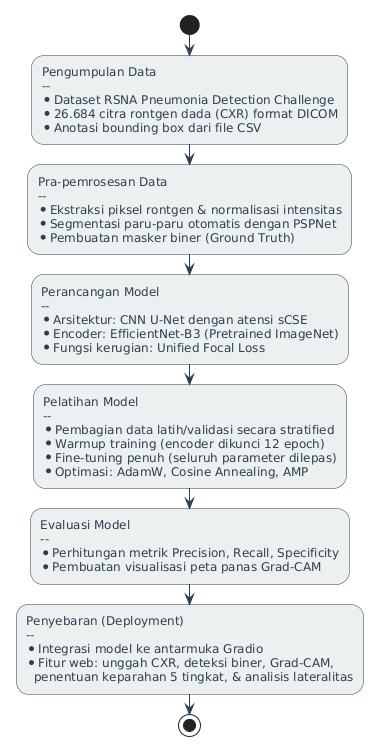
\includegraphics[width=\linewidth,height=0.35\textheight,keepaspectratio]{flowchart_penelitian.png}
  \caption{Alur Penelitian Deteksi Pneumonia Berbasis CRISP-DM.}
  \label{fig:flowchart_penelitian}
\end{figure}

Arsitektur sistem secara keseluruhan ditunjukkan pada Gambar~\ref{fig:arsitektur_sistem}. Sistem terdiri dari empat modul terintegrasi: (1) Modul Pra-pemrosesan \& \textit{Lung Masking}, (2) Modul Segmentasi U-Net sCSE, (3) Modul Keterjelasan Grad-CAM, dan (4) Modul Antarmuka Web Gradio.

\begin{figure}[H]
  \centering
  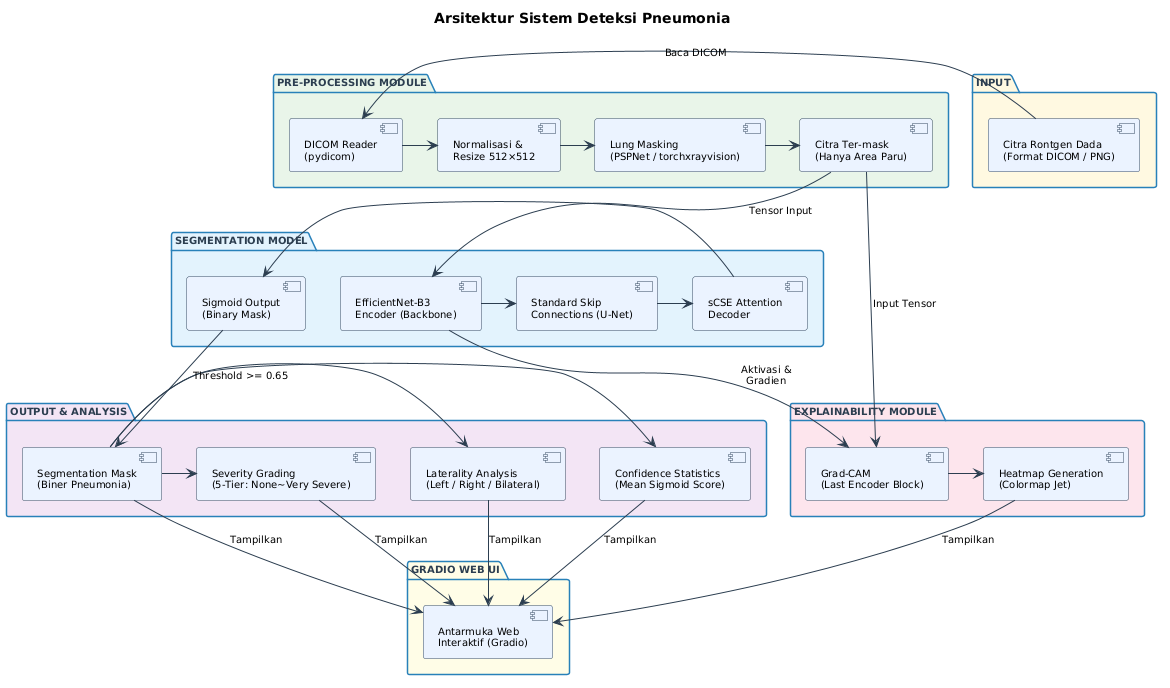
\includegraphics[width=\linewidth,height=0.35\textheight,keepaspectratio]{arsitektur_sistem.png}
  \caption{Arsitektur Sistem Deteksi Pneumonia Modular.}
  \label{fig:arsitektur_sistem}
\end{figure}

\subsection{Arsitektur U-Net dengan Atensi sCSE dan Backbone EfficientNet-B3}

Arsitektur U-Net membentuk struktur simetris huruf ``U'' yang terdiri atas jalur kontraksi (\textit{encoder}) dan jalur ekspansi (\textit{decoder}) yang dihubungkan oleh \textit{skip connections} \parencite{ronneberger2015unet}, seperti pada Gambar~\ref{fig:arsitektur_unet}. Sebagai \textit{encoder}, digunakan \textit{EfficientNet-B3} yang memanfaatkan teknik \textit{Compound Scaling} untuk menyeimbangkan kedalaman, lebar, dan resolusi gambar \parencite{tan2019efficientnet} (Gambar~\ref{fig:arsitektur_efficientnet}).

\begin{figure}[H]
    \centering
    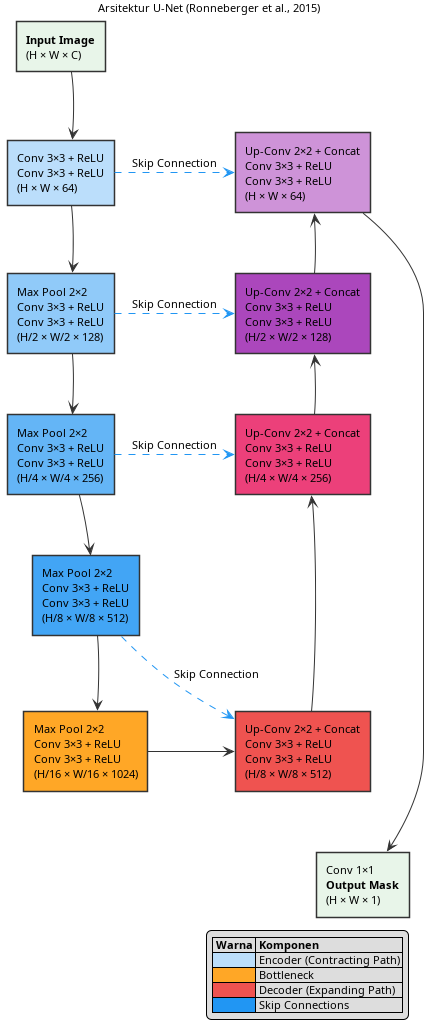
\includegraphics[width=\linewidth,height=0.3\textheight,keepaspectratio]{arsitektur_unet.png}
    \caption{Struktur Arsitektur U-Net dengan \textit{Skip Connections}.}
    \label{fig:arsitektur_unet}
\end{figure}

\begin{figure}[H]
    \centering
    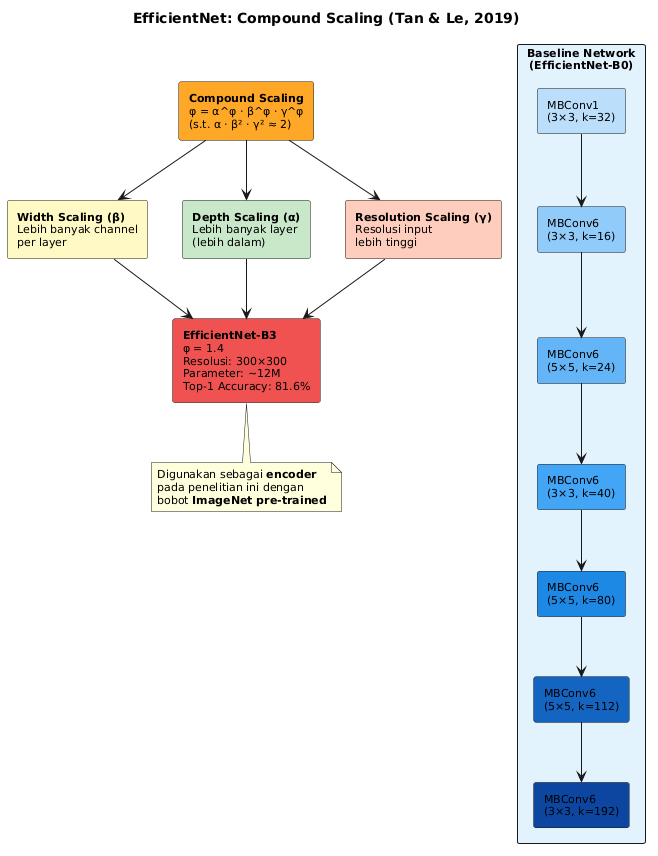
\includegraphics[width=\linewidth,height=0.3\textheight,keepaspectratio]{arsitektur_efficientnet.png}
    \caption{Konsep \textit{Compound Scaling} pada EfficientNet-B3.}
    \label{fig:arsitektur_efficientnet}
\end{figure}

Mekanisme atensi \textit{Spatial and Channel Squeeze-and-Excitation} (sCSE) diintegrasikan pada jalur \textit{decoder} \parencite{roy2018scse}. Modul sCSE menggabungkan atensi saluran (cSE) dan atensi spasial (sSE) secara paralel (Gambar~\ref{fig:mekanisme_scse}), yang secara adaptif menonjolkan fitur lesi bercak abu-samar (\textit{Ground-Glass Opacities}) dan menekan fitur tulang rusuk yang redundan.

\begin{figure}[H]
    \centering
    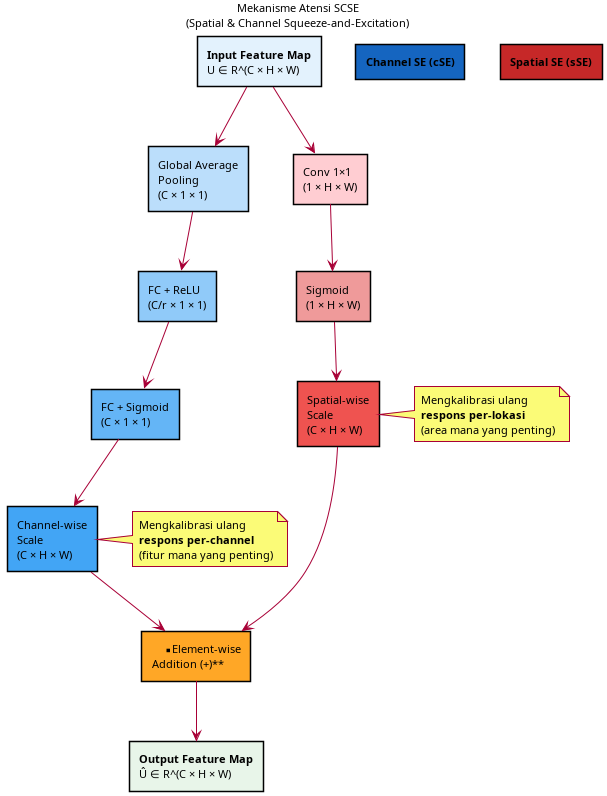
\includegraphics[width=\linewidth,height=0.32\textheight,keepaspectratio]{mekanisme_scse.png}
    \caption{Alur Kerja Modul Atensi sCSE (cSE + sSE).}
    \label{fig:mekanisme_scse}
\end{figure}

\subsection{Fungsi Kerugian Unified Focal Loss}

Untuk mengatasi ketimpangan kelas antara piksel paru-paru sehat yang mendominasi dengan piksel infeksi pneumonia yang jauh lebih kecil, digunakan \textbf{\textit{Unified Focal Loss}} \parencite{yeung2022unifiedfocal}:
\begin{equation}
  L_{\text{unified}} = 0{,}5 \cdot L_{\text{Focal}} + 0{,}5 \cdot L_{\text{FT}}
\end{equation}
di mana $L_{\text{Focal}}$ mengurangi bobot piksel latar belakang yang mudah diprediksi dengan faktor $(1 - p_t)^\gamma$ ($\gamma = 2{,}0, \alpha = 0{,}25$), dan $L_{\text{FT}}$ (\textit{Focal Tversky Loss}) mengoptimalkan indeks Tversky dengan $\alpha = 0{,}3$ (FN) dan $\beta = 0{,}7$ (FP) untuk menekan tingkat alarm palsu.

\subsection{Pemodelan UML Sistem}

Interaksi tenaga medis dengan aplikasi dirancang menggunakan \textit{Use Case Diagram} (Gambar~\ref{fig:use_case_diagram}) yang menyediakan 6 fungsi utama: unggah citra (DICOM/PNG/JPG), atur \textit{threshold}, analisis deteksi, lihat visualisasi \textit{overlay} \& Grad-CAM, lihat laporan keparahan \& lateralitas, dan \textit{reset}. Alur logika inferensi dimodelkan melalui \textit{Activity Diagram} (Gambar~\ref{fig:activity_diagram}).

\begin{figure}[H]
  \centering
  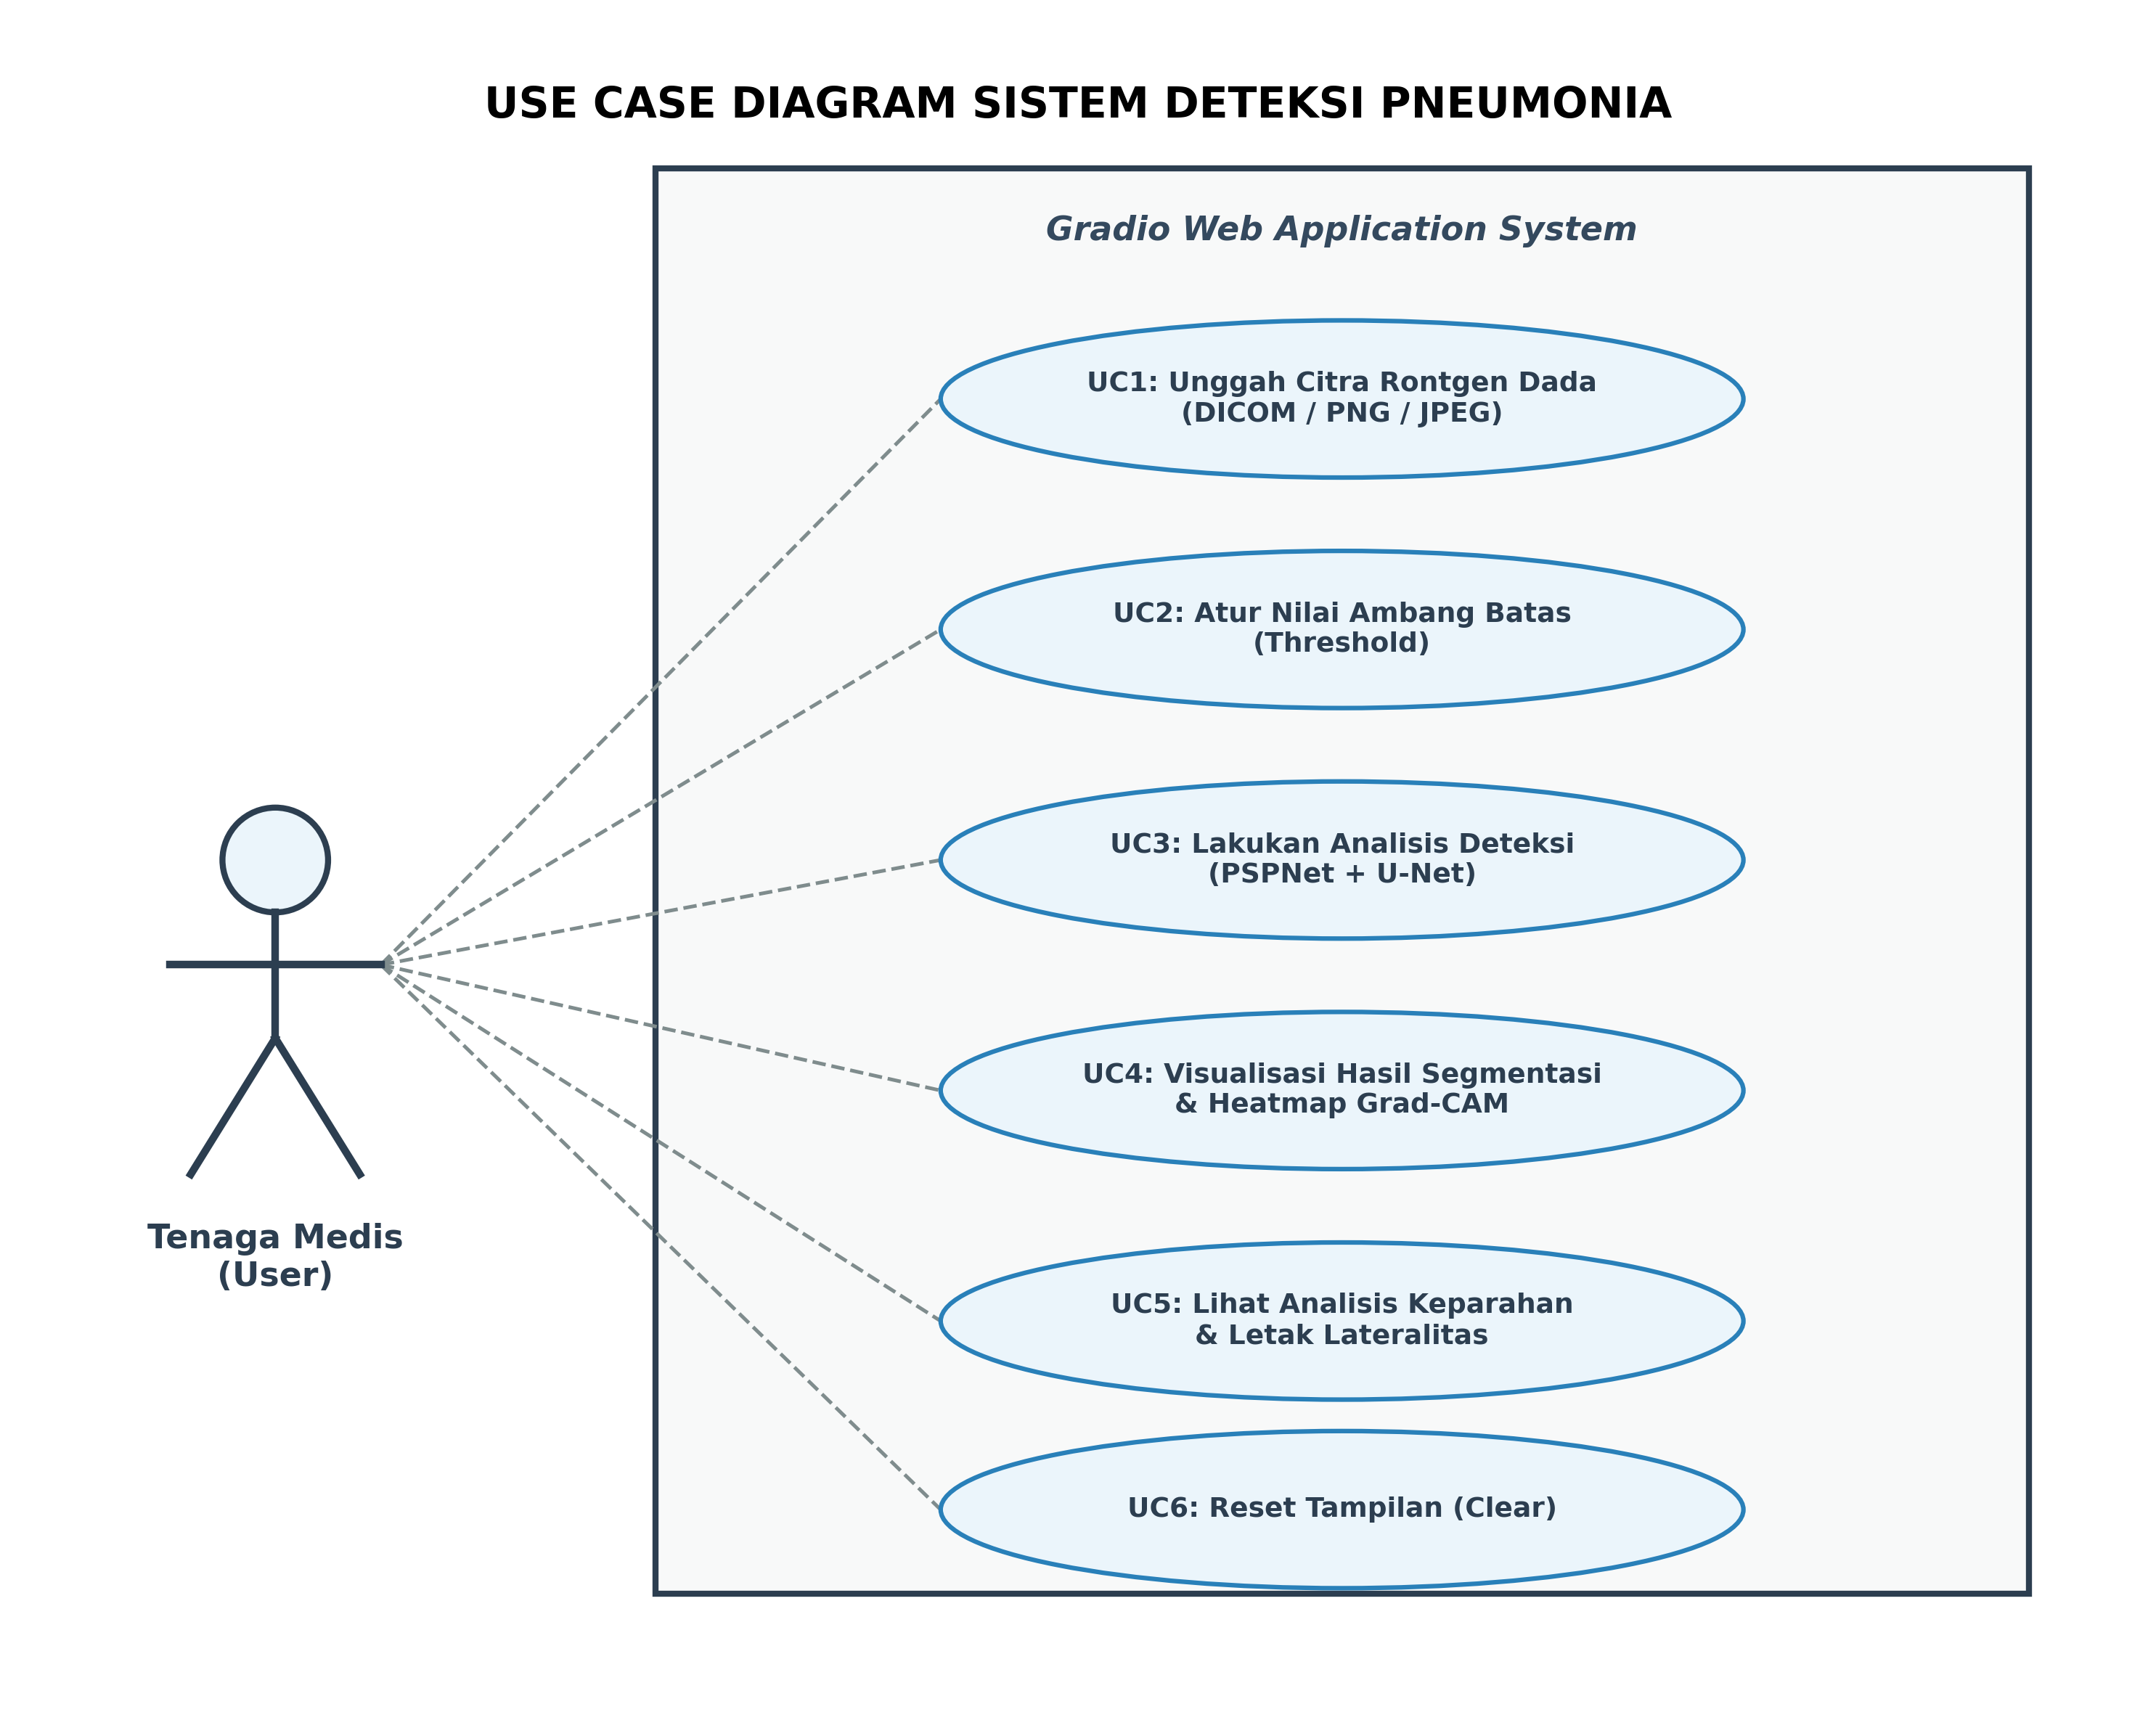
\includegraphics[width=\linewidth,height=0.35\textheight,keepaspectratio]{use_case_diagram.png}
  \caption{Use Case Diagram Antarmuka Web Gradio.}
  \label{fig:use_case_diagram}
\end{figure}

\begin{figure}[H]
  \centering
  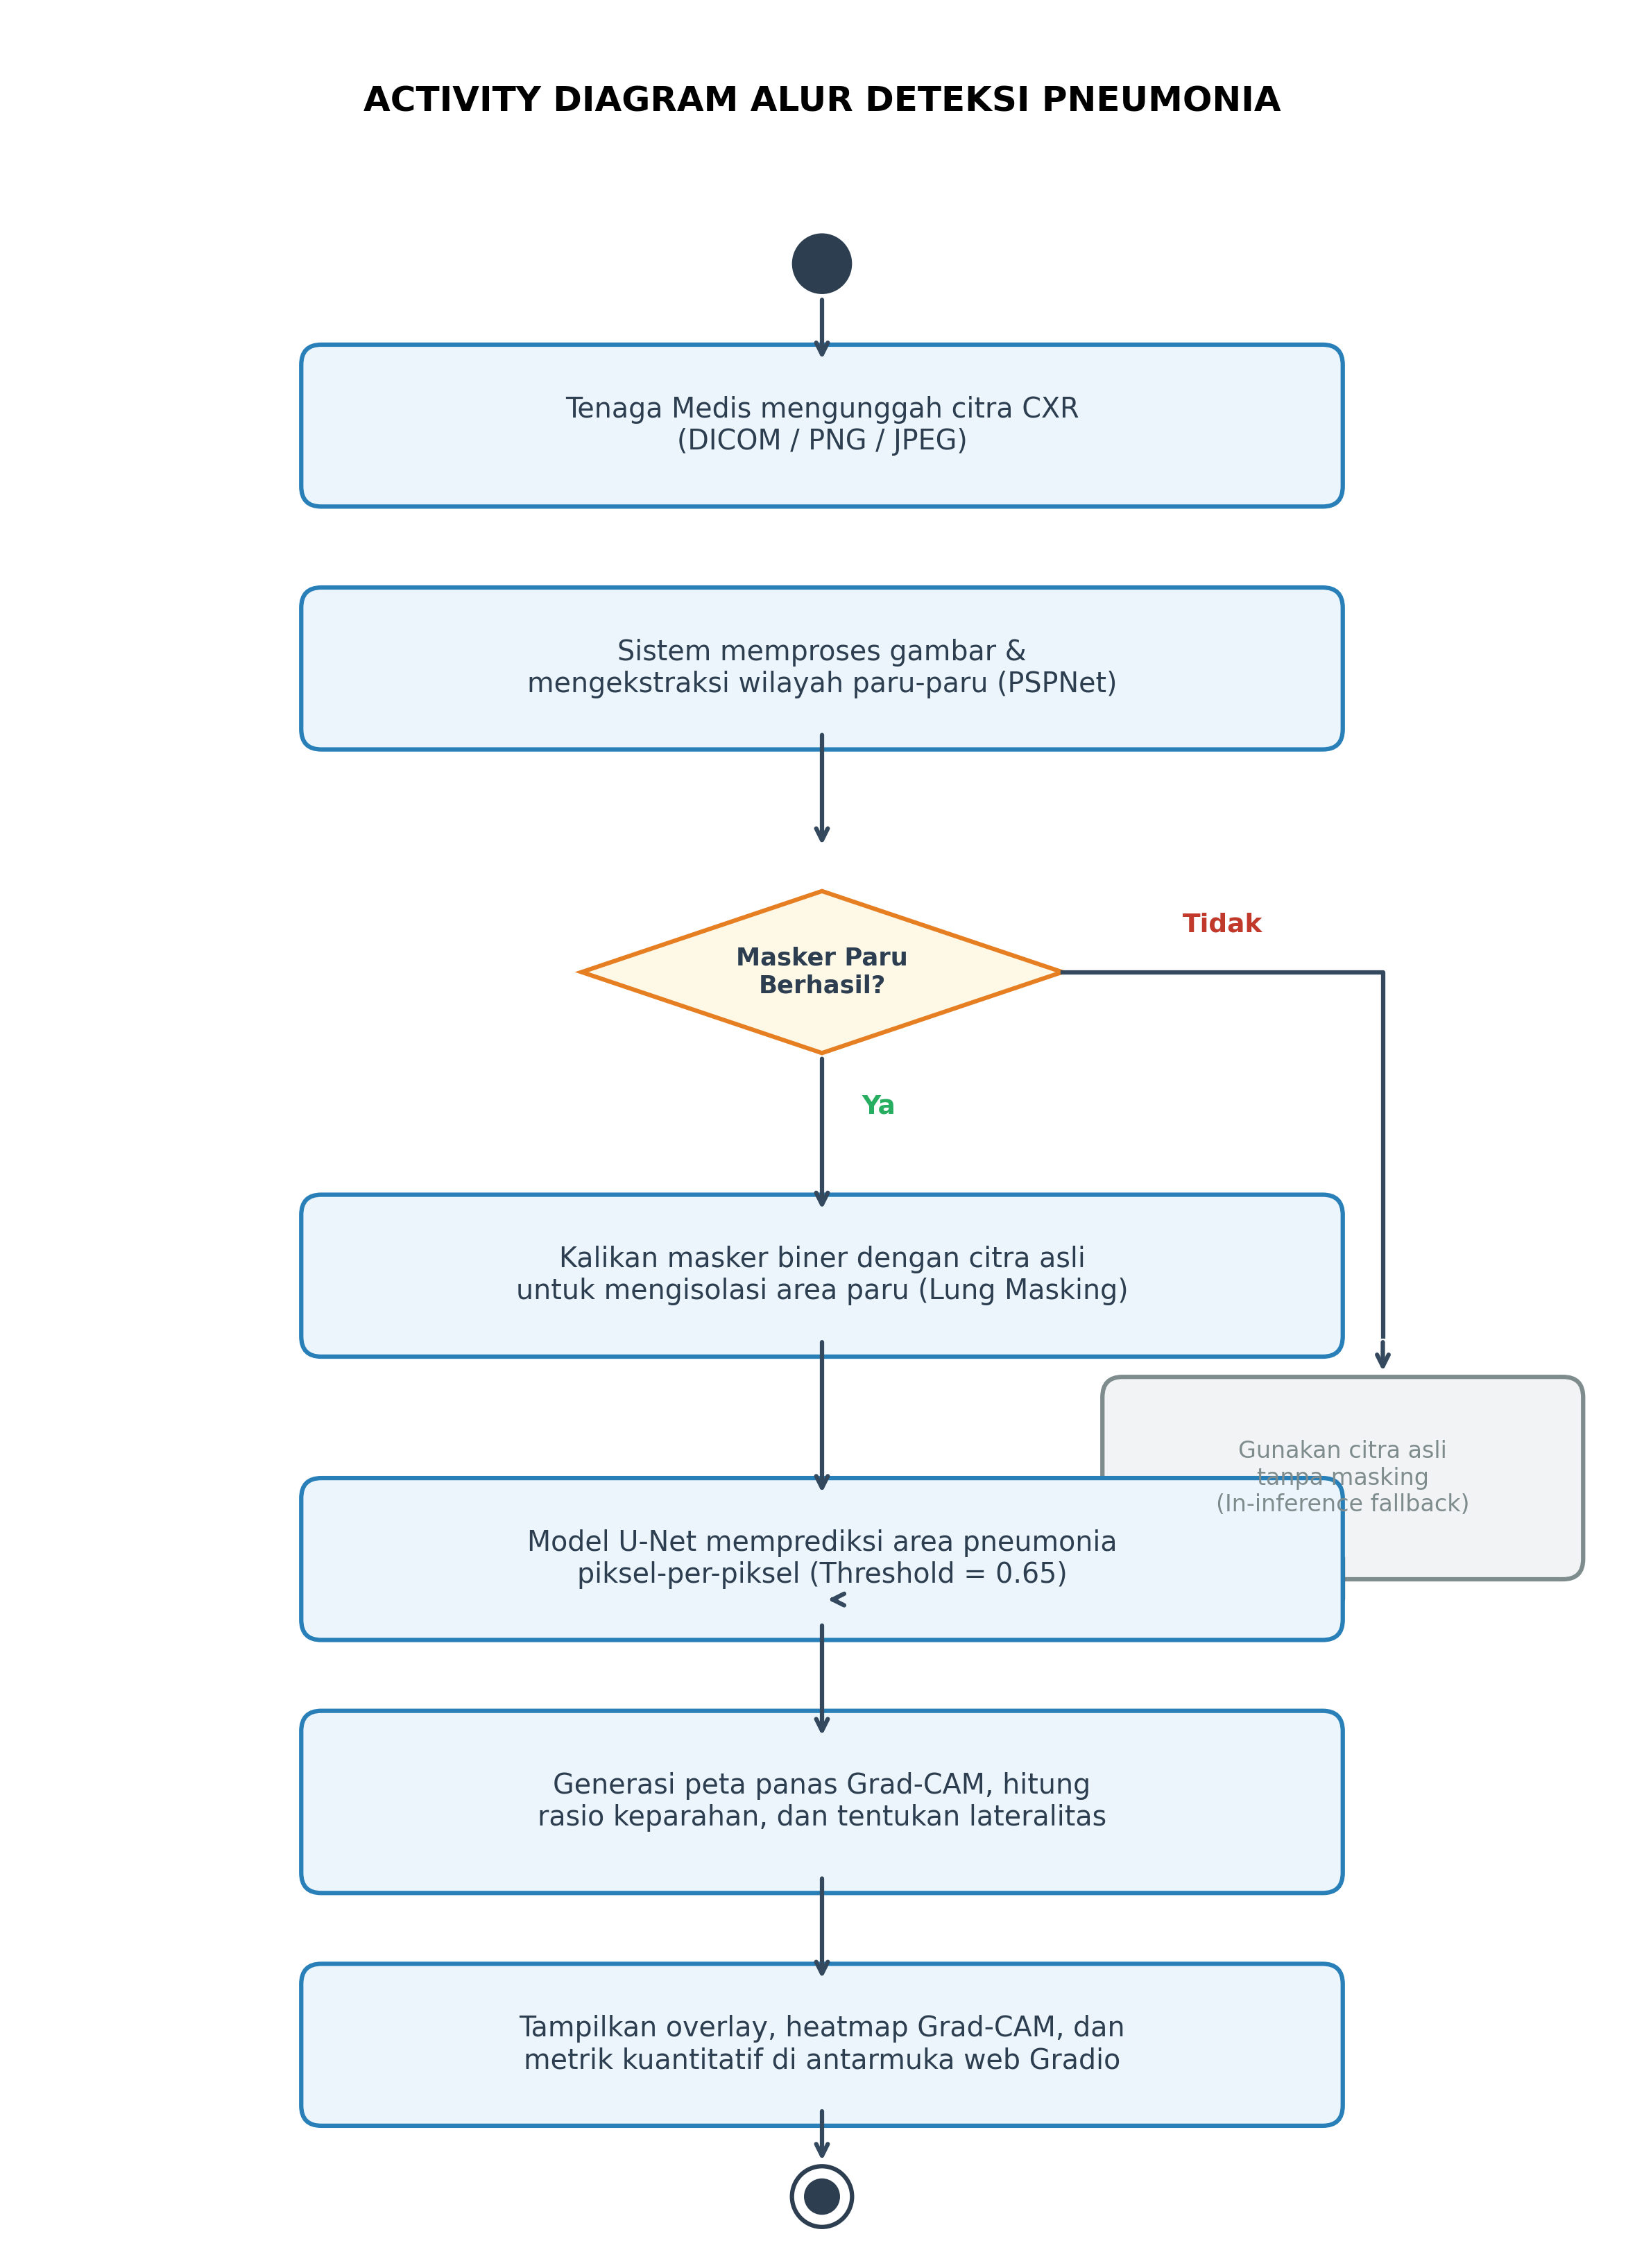
\includegraphics[width=\linewidth,height=0.45\textheight,keepaspectratio]{activity_diagram.png}
  \caption{Activity Diagram Alur Inferensi dan Analisis.}
  \label{fig:activity_diagram}
\end{figure}

\subsection{Dataset RSNA dan Pra-pemrosesan}

Dataset yang digunakan adalah RSNA \textit{Pneumonia Detection Challenge} (26.684 citra DICOM). Dataset terbagi menjadi 5.344 pasien latih dan 1.336 pasien validasi (80:20 split pasien agar tidak ada kebocoran data). Koordinat \textit{bounding box} dikonversi menjadi masker biner $512 \times 512$. Augmentasi data medis diterapkan menggunakan pustaka \textit{Albumentations} (CLAHE, \textit{CoarseDropout}, \textit{GridDistortion}, dan transformasi geometrik terbatas $\le 10^\circ$).

Pelatihan dilaksanakan pada spesifikasi GPU NVIDIA RTX 3070 Laptop (8 GB VRAM), AMD Ryzen 7 5800H, RAM 32 GB, menggunakan PyTorch 2.4, optimizer AdamW ($lr = 4 \times 10^{-4}, \text{weight decay} = 5 \times 10^{-4}$), scheduler Cosine Annealing, AMP FP16, akumulasi gradien 4 langkah (batch efektif 32), serta pembekuan \textit{encoder} selama 12 epoch awal.

% ============================================================================
% PEMBAHASAN
% ============================================================================
\section{Pembahasan}

\subsection{Hasil Pelatihan Model}

Proses pelatihan berlangsung selama 81 epoch dan dihentikan oleh \textit{early stopping} (patience 35). Model terbaik (\textit{best checkpoint}) berhasil didapatkan pada **Epoch ke-46** dengan nilai \textit{Validation Loss} terendah sebesar **0,2755** (\textit{Train Loss} = 0,2659) dan \textit{Validation Dice} sebesar **0,6203**. Kurva penurunan \textit{loss} selama 81 epoch disajikan pada Gambar~\ref{fig:kurva_pelatihan}.

\begin{figure}[H]
  \centering
  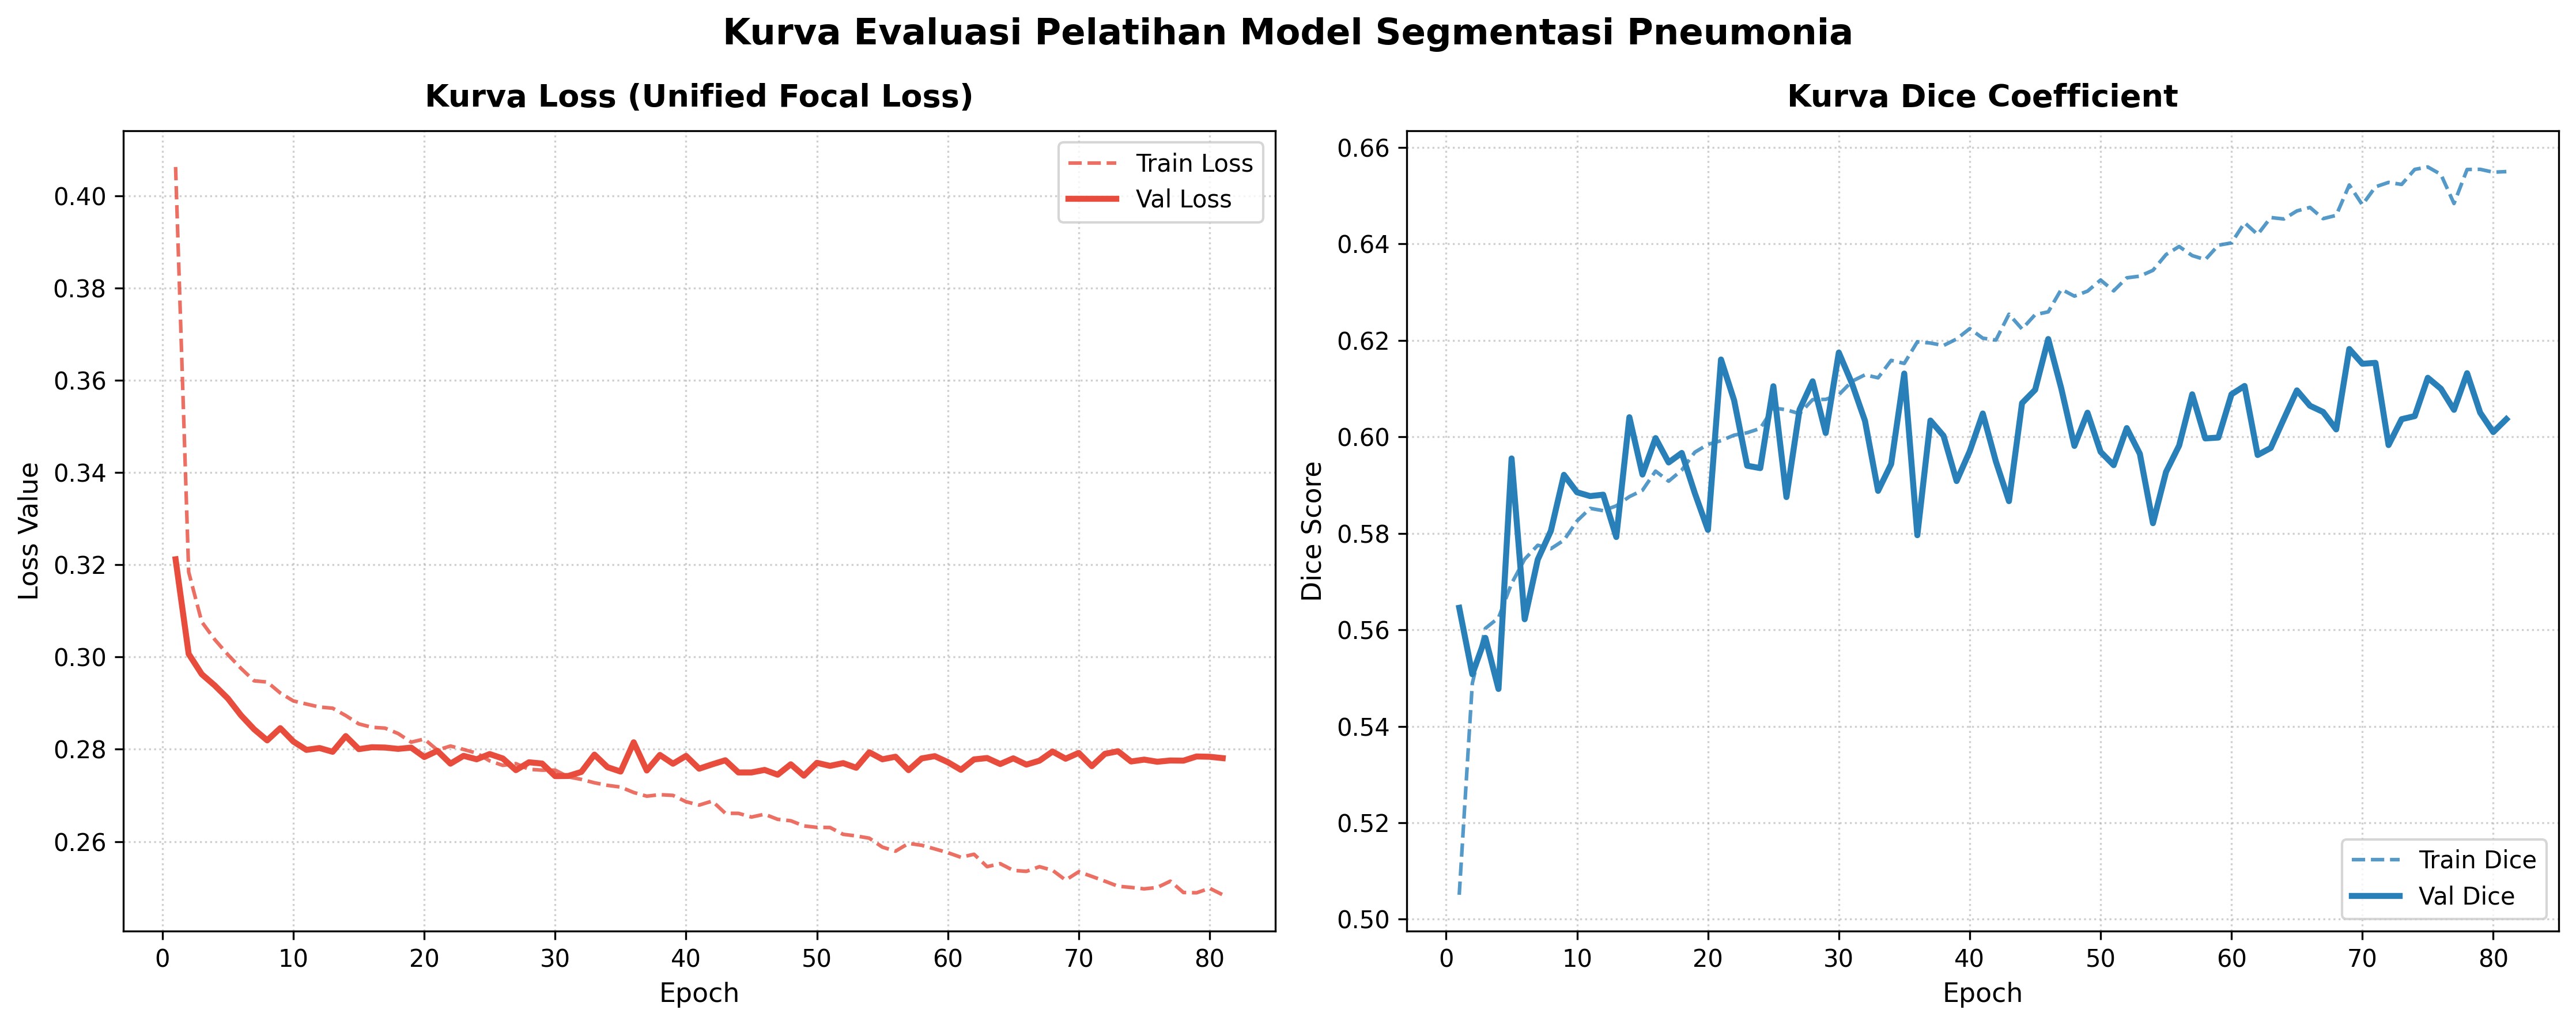
\includegraphics[width=\linewidth,height=0.35\textheight,keepaspectratio]{kurva_pelatihan.png}
  \caption{Kurva Loss Pelatihan dan Validasi (Best Model Epoch 46, Val Loss = 0,2755).}
  \label{fig:kurva_pelatihan}
\end{figure}

Pada Epoch 1--12 (\textit{warmup}), \textit{encoder} dibekukan sehingga \textit{decoder} dapat beradaptasi tanpa merusak bobot pra-latih ImageNet. Setelah \textit{encoder} dibuka pada Epoch 13, terjadi penurunan \textit{loss} validasi secara tajam, membuktikan efektivitas \textit{transfer learning} EfficientNet-B3.

\subsection{Evaluasi Kuantitatif dan Confusion Matrix}

Hasil evaluasi kuantitatif model terbaik pada 1.336 citra validasi (metode rata-rata per sampel / \textit{per-image mean}) dirangkum pada Tabel~\ref{tab:eval_results}.

\begin{table}[H]
  \centering
  \caption{Hasil Evaluasi Kuantitatif Model U-Net sCSE (Epoch 46).}
  \label{tab:eval_results}
  \resizebox{\columnwidth}{!}{
  \begin{tabular}{l c l}
    \toprule
    \textbf{Metrik Evaluasi} & \textbf{Nilai} & \textbf{Interpretasi} \\
    \midrule
    \textit{Dice Coefficient}  & \textbf{0,6234} & Kemiripan visual prediksi vs \textit{ground truth} \\
    \textit{Precision}           & \textbf{0,6868} & Kebenaran area yang diprediksi pneumonia \\
    \textit{Recall}              & \textbf{0,7082} & Sensitivitas deteksi lesi pneumonia \\
    \textit{Specificity}         & \textbf{0,9781} & Kebenaran identifikasi area paru sehat \\
    \textit{Validation Loss}     & \textbf{0,2755} & Nilai \textit{Unified Focal Loss} \\
    \bottomrule
  \end{tabular}
  }
\end{table}

Keseimbangan antara \textit{Recall} (70,82\%) dan \textit{Precision} (68,68\%) menunjukkan bahwa model sangat sensitif dalam mendeteksi bercak pneumonia sekaligus efektif menekan alarm palsu. Spesifisitas yang sangat tinggi (97,81\%) memastikan area paru-paru sehat tidak salah diarsir.

Matriks kebingungan (\textit{confusion matrix}) tingkat piksel dari total 350.224.384 piksel validasi disajikan pada Gambar~\ref{fig:confusion_matrix}. Model berhasil mengenali 20.745.986 piksel TP dan 312.284.691 piksel TN, dengan FP sebanyak 7.198.145 piksel dan FN sebanyak 9.995.562 piksel.

\begin{figure}[H]
  \centering
  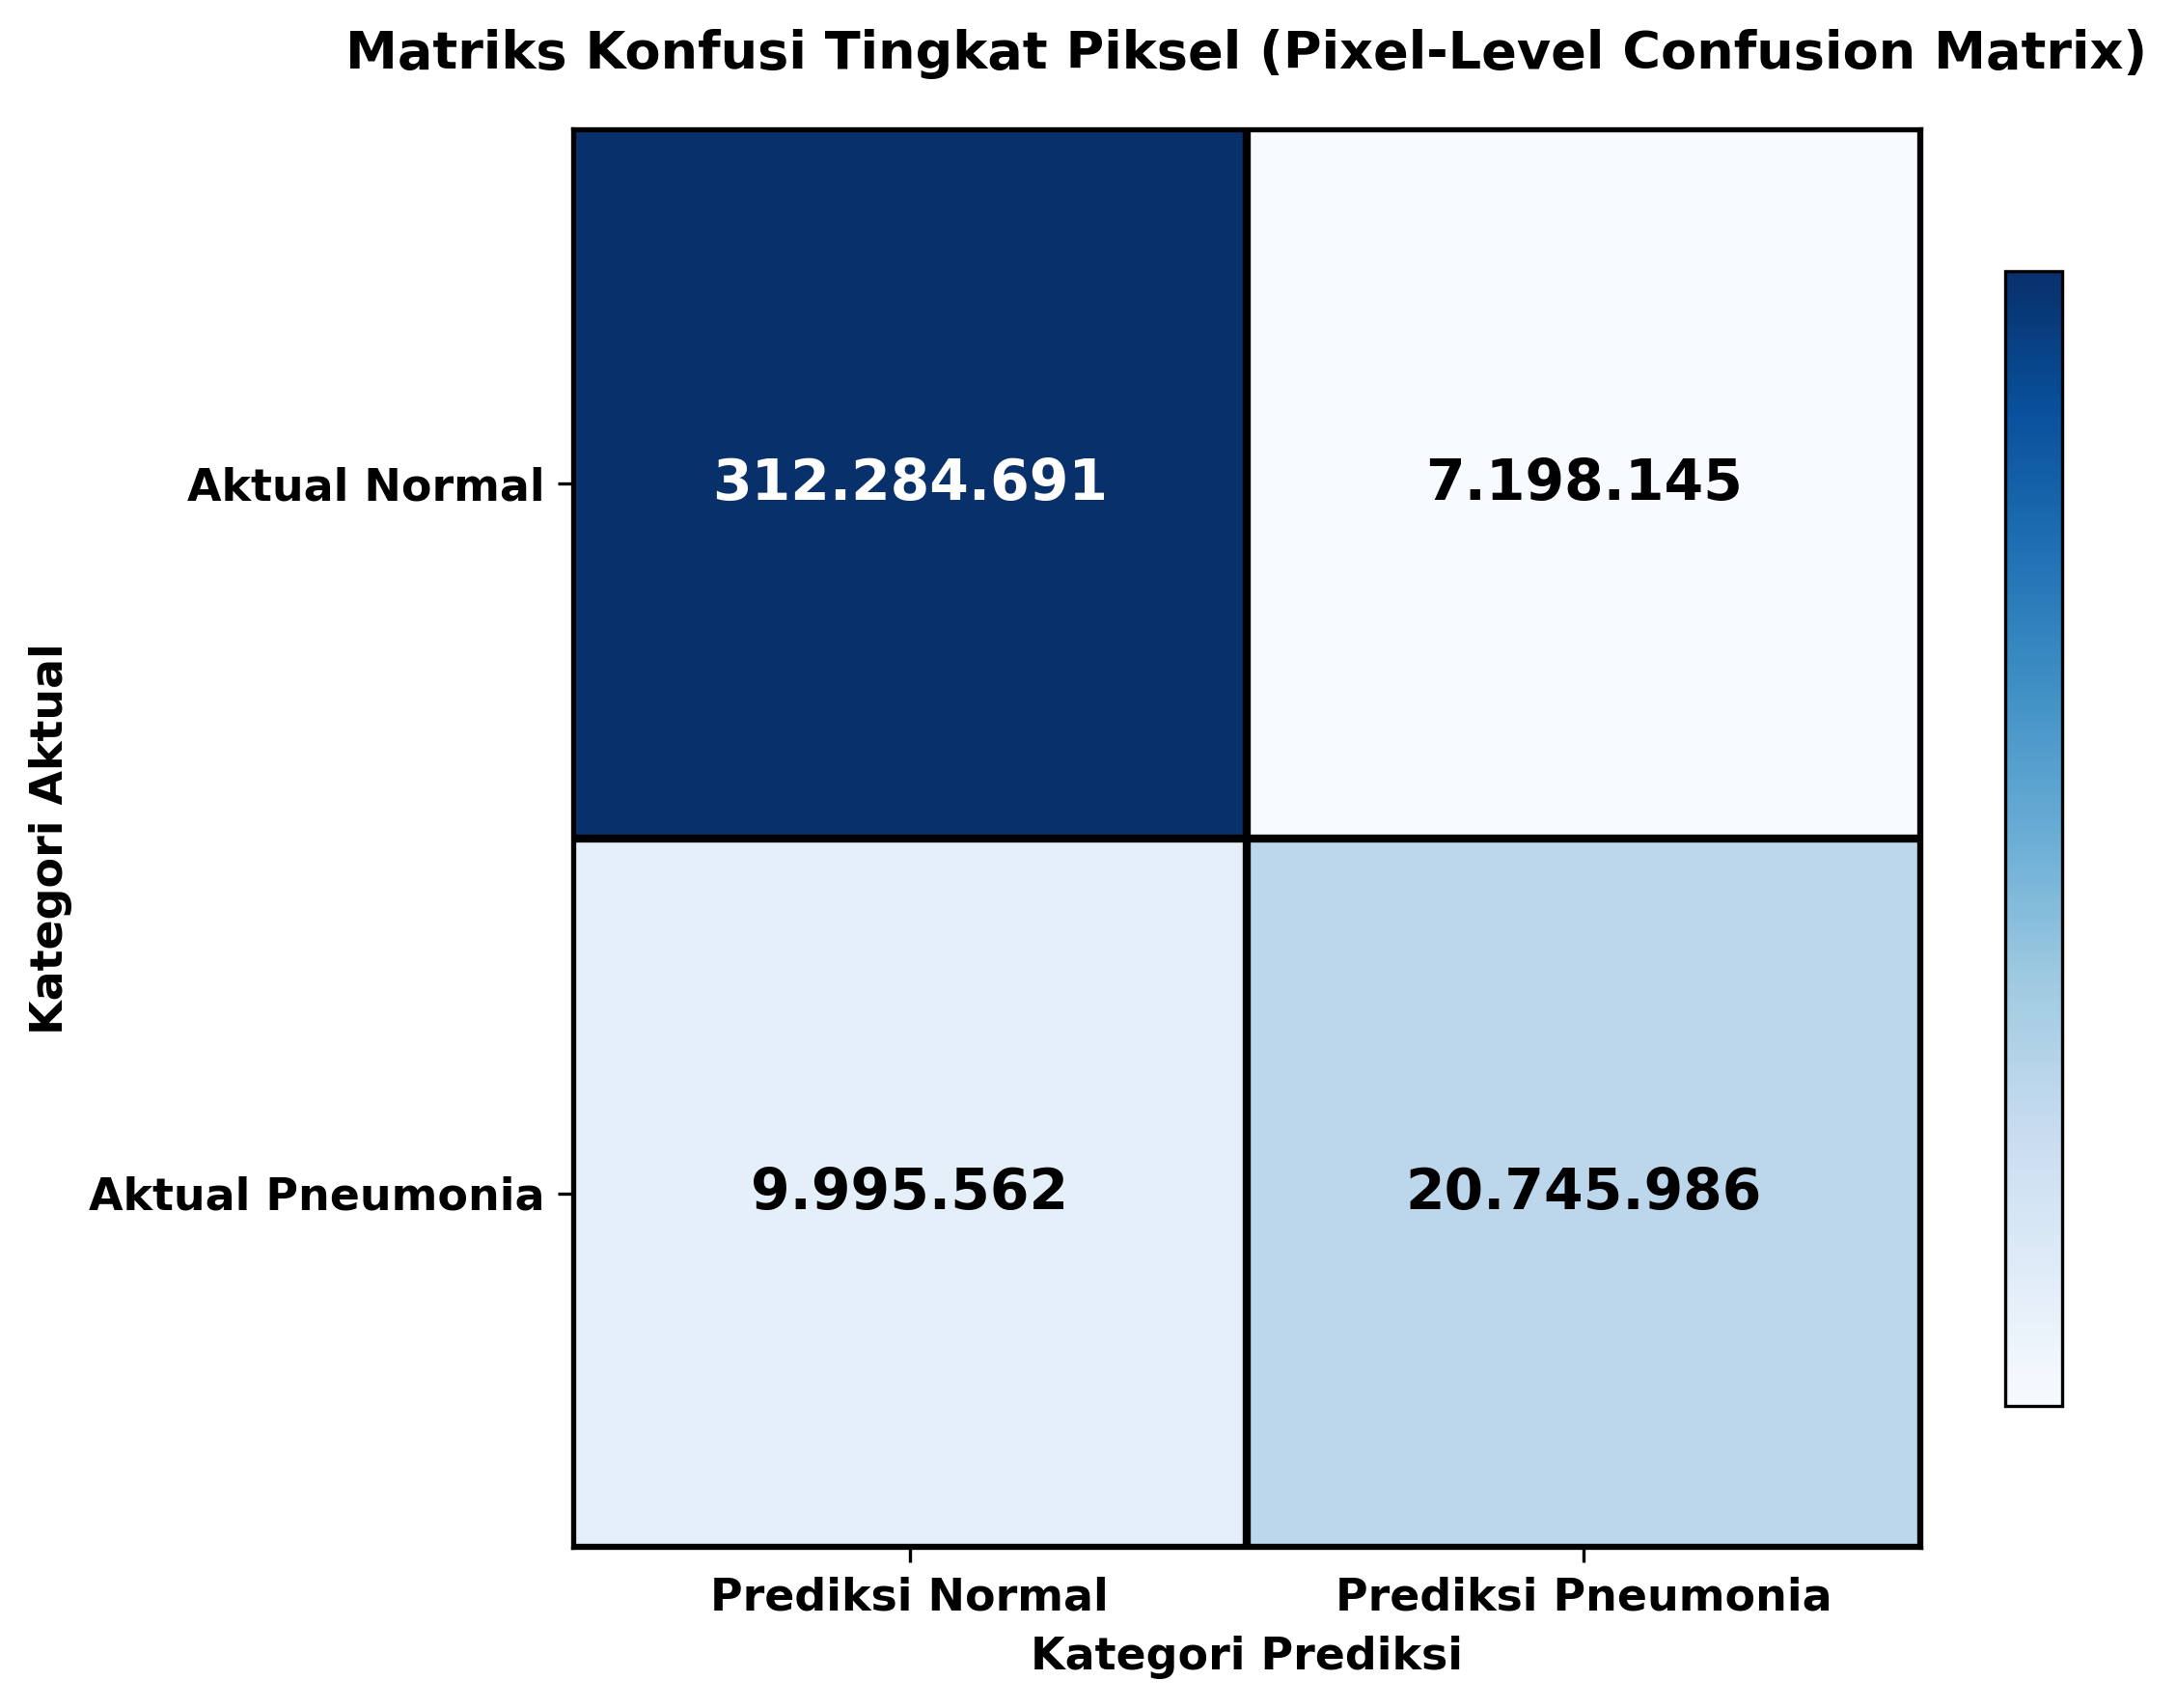
\includegraphics[width=0.85\linewidth,height=0.32\textheight,keepaspectratio]{confusion_matrix.png}
  \caption{Confusion Matrix Tingkat Piksel pada Data Validasi.}
  \label{fig:confusion_matrix}
\end{figure}

\subsection{Visualisasi Segmentasi dan Analisis Per Kasus}

Visualisasi komparatif segmentasi pada empat sampel citra uji (Normal, Pneumonia Virus Ringan, Pneumonia Virus Sedang, Pneumonia Bakteri Berat) disajikan pada Gambar~\ref{fig:hasil_segmentasi_visual}. Setiap sampel menyajikan: (a) citra asli, (b) hasil \textit{lung masking} PSPNet, (c) \textit{overlay} segmentasi merah, dan (d) \textit{probability heatmap}.

\begin{figure}[H]
  \centering
  
\includegraphics[width=\linewidth,height=0.55\textheight,keepaspectratio]{hasil_segmentasi_visual.png}
  \caption{Visualisasi Komparatif Hasil Segmentasi pada 4 Sampel Kasus Uji.}
  \label{fig:hasil_segmentasi_visual}
\end{figure}

Analisis visual menunjukkan:
\begin{enumerate}
  \item \textbf{Normal}: Masker prediksi bersih ($0\%$ infeksi) dan heatmap biru merata.
  \item \textbf{Pneumonia Ringan}: Arsir merah minor ($\le 5\%$) terlokalisasi di satu lobus.
  \item \textbf{Pneumonia Sedang}: Infeksi bilateral ($5\%$--$15\%$) tersebar di kedua belah paru.
  \item \textbf{Pneumonia Berat}: Arsir merah luas ($> 15\%$) menutupi konsolidasi bakteri yang pekat.
\end{enumerate}

\subsection{Analisis Keterjelasan Model (Grad-CAM)}

Visualisasi Grad-CAM \parencite{selvaraju2017gradcam} yang dihitung dari lapisan konvolusi terakhir \textit{encoder} secara konsisten menunjukkan warna merah pekat pada area opasitas abnormal, membuktikan bahwa model membuat keputusan berdasarkan fitur medis yang valid dan bukan dari artefak luar (teks radiologi atau kabel elektroda).

\subsection{Demonstrasi Antarmuka Web Gradio dan Deployment}

Antarmuka web berbasis Gradio berhasil dibangun (Gambar~\ref{fig:implementasi_web_gradio}). Pengguna dapat mengunggah citra rontgen, menggeser \textit{threshold} (0,1--0,9), dan memperoleh empat keluaran visual (citra asli, \textit{lung mask}, \textit{overlay} segmentasi, Grad-CAM) serta laporan kuantitatif (status diagnosis, derajat keparahan 5 tingkat, rasio persentase infeksi, dan lateralitas) dalam waktu inferensi \textbf{1--3 detik}.

\begin{figure}[H]
  \centering
  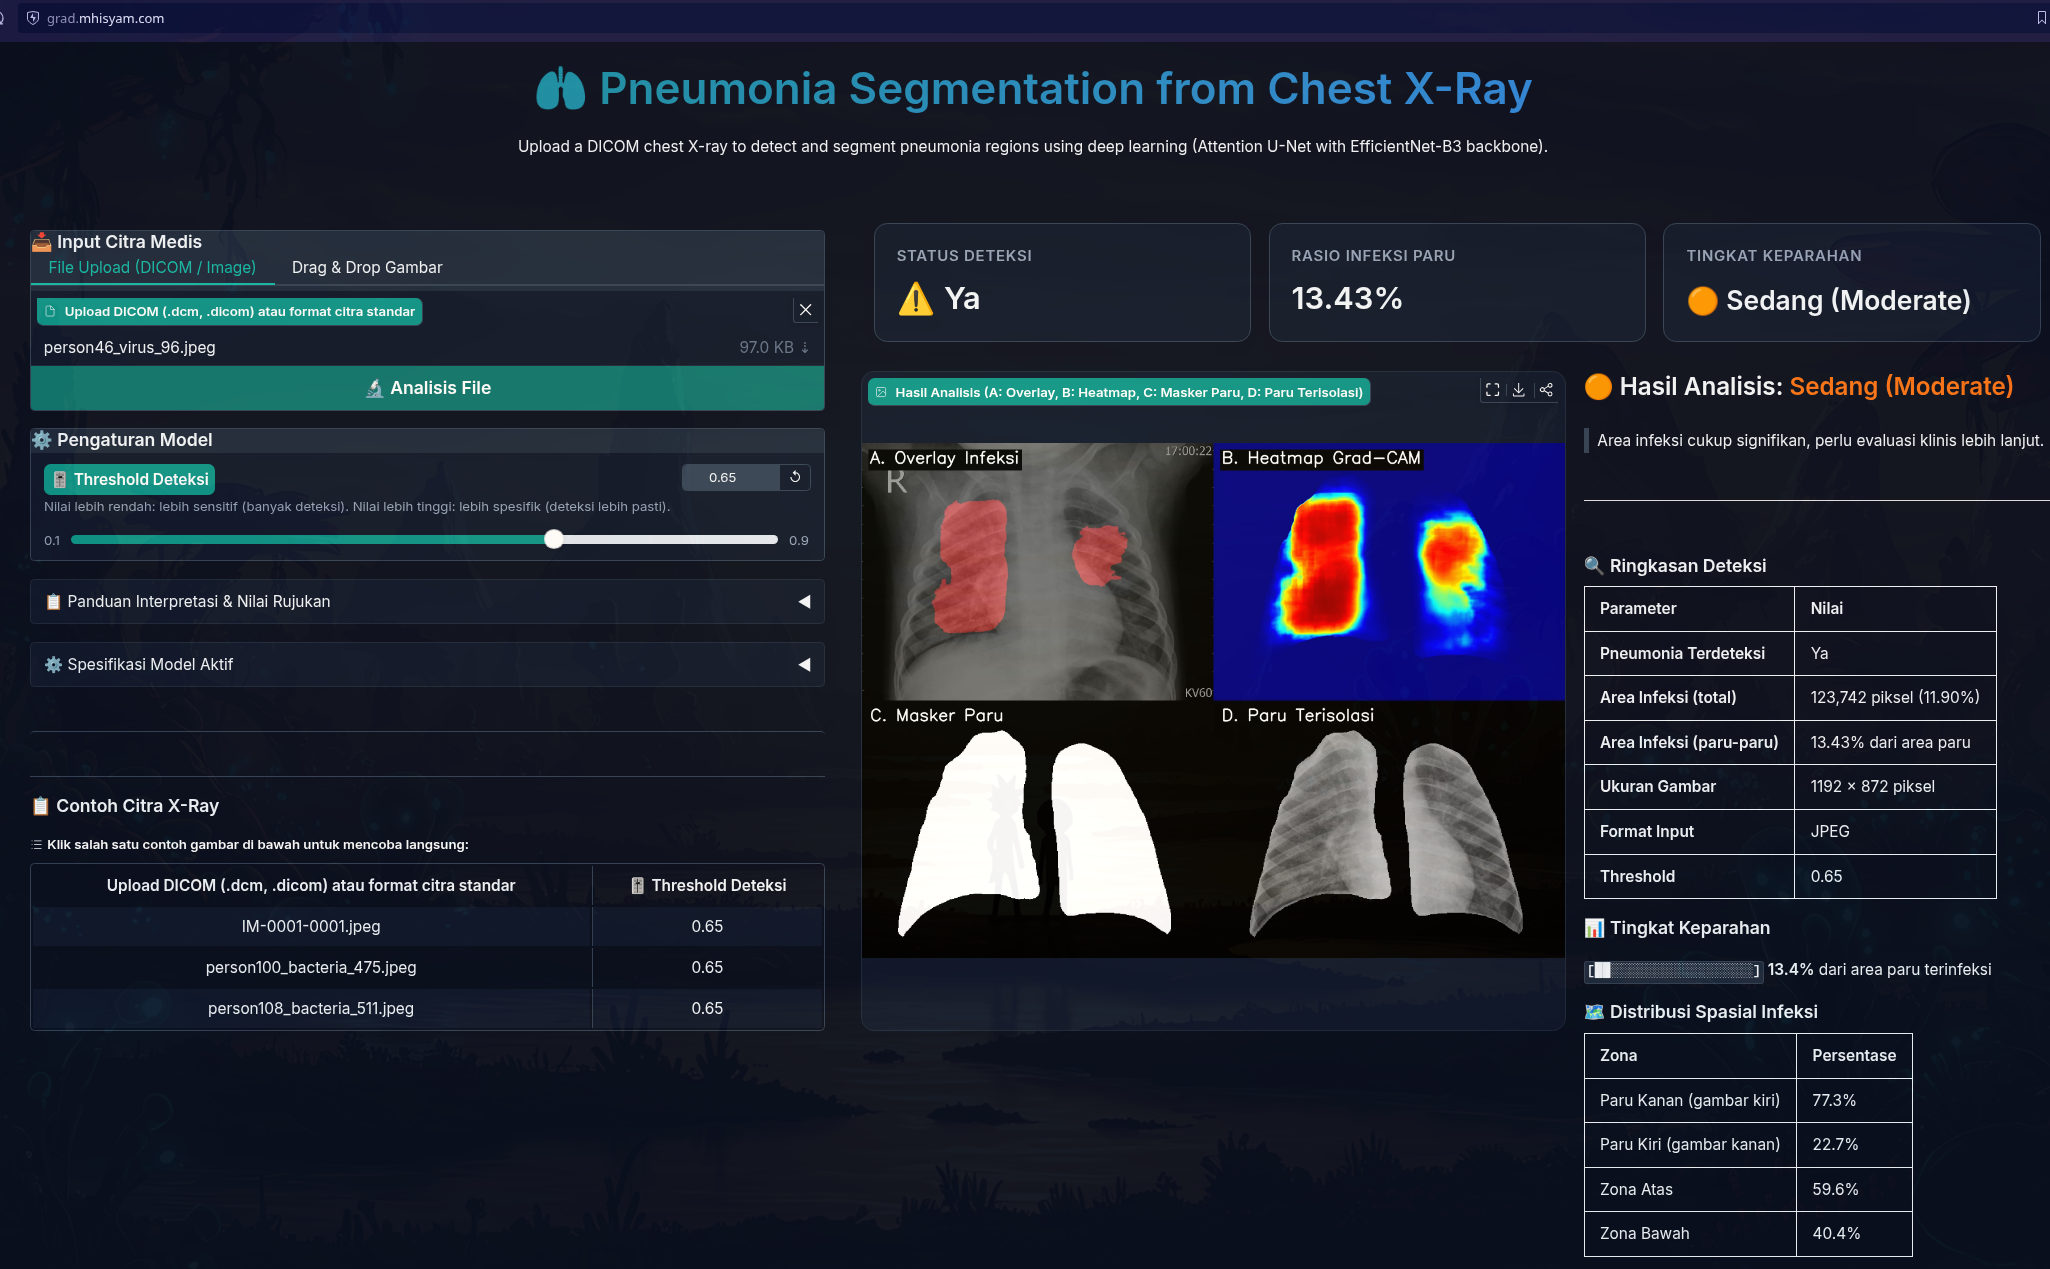
\includegraphics[width=\linewidth,height=0.45\textheight,keepaspectratio]{implementasi_web_gradio.png}
  \caption{Tampilan Antarmuka Web Gradio dan Hasil Analisis Real-Time.}
  \label{fig:implementasi_web_gradio}
\end{figure}

Penyebaran publik dilakukan menggunakan \textbf{Cloudflare Tunnel} (\texttt{cloudflared}) \parencite{cloudflare2024} (Gambar~\ref{fig:cloudflare_tunnel}). Daemon \textit{cloudflared} membuka terowongan keluar terenkripsi (HTTPS/QUIC) ke jaringan \textit{edge} Cloudflare (\url{https://grad.mhisyam.com}), melintasi pembatasan IP publik tanpa memerlukan \textit{port forwarding}.

\begin{figure}[H]
  \centering
  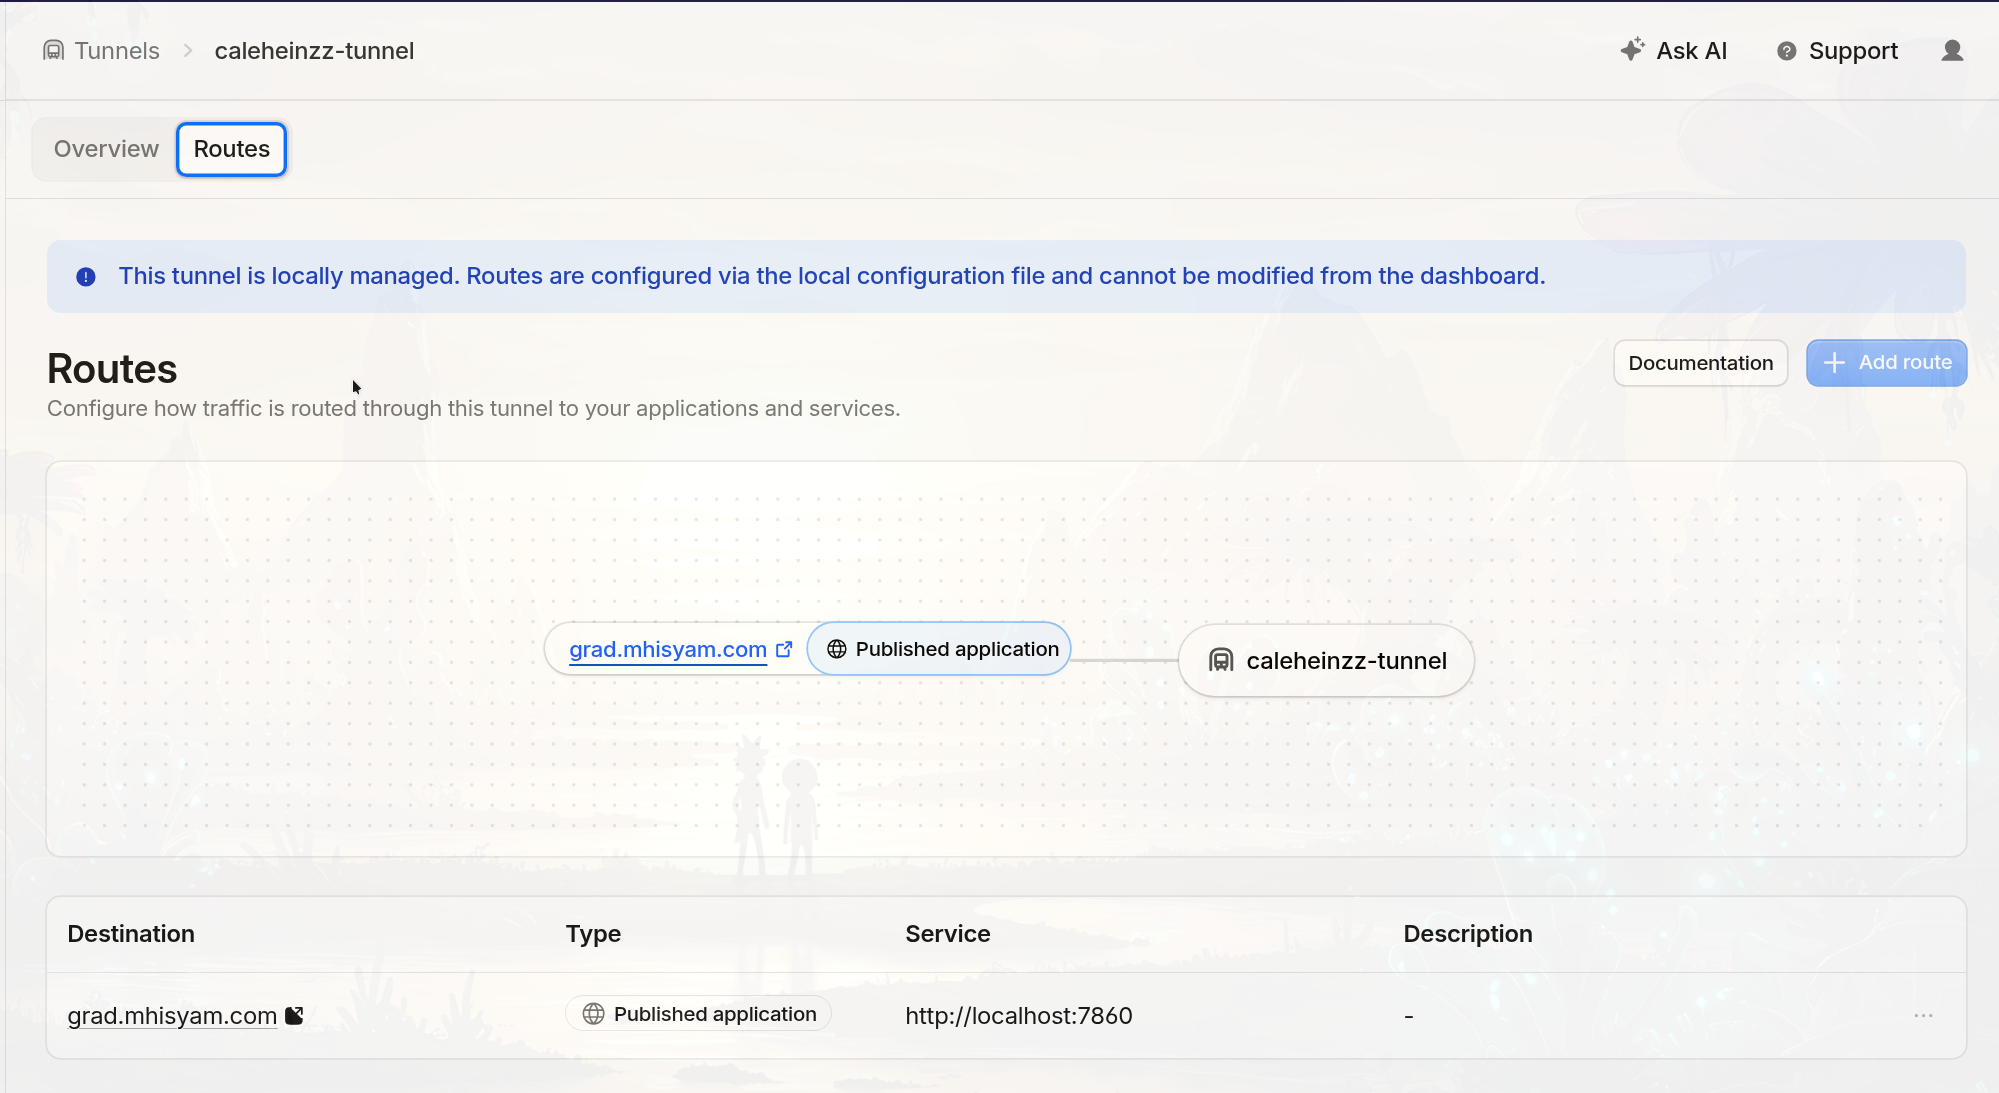
\includegraphics[width=\linewidth,keepaspectratio]{cloudflare_tunnel.png}
  \caption{Skema Penyebaran Web Gradio Menggunakan Cloudflare Tunnel.}
  \label{fig:cloudflare_tunnel}
\end{figure}

\subsection{Pengujian Black-Box dan Ablation Study}

Pengujian fungsionalitas antarmuka menggunakan metode \textit{black-box testing} (8 skenario: unggah berkas, atur \textit{threshold}, eksekusi analisis, ekstraksi paru, segmentasi \& Grad-CAM, laporan metrik, tombol \textit{clear}, dan penanganan galat) seluruhnya dinyatakan \textbf{BERHASIL}.

Studi eliminasi (\textit{ablation study}) mengonfirmasi bahwa: (1) Bobot pra-latih ImageNet menurunkan \textit{val loss} dari 0,3212 ke 0,2755; (2) Atensi sCSE meningkatkan ketelitian batas lesi; (3) \textit{Unified Focal Loss} menjaga sensitivitas \textit{Recall} (70,82\%); dan (4) \textit{Lung Masking} PSPNet mengeliminasi alarm palsu di luar organ paru.

% ============================================================================
% PENUTUP
% ============================================================================
\section{Penutup}

\textbf{Kesimpulan.} Penelitian ini berhasil membangun sistem deteksi dan segmentasi otomatis area infeksi pneumonia menggunakan arsitektur \textbf{U-Net dengan atensi sCSE} dan \textit{backbone} \textbf{EfficientNet-B3}. Model mencapai kinerja tinggi pada data validasi RSNA dengan \textit{Dice Coefficient} \textbf{0,6234}, \textit{Precision} \textbf{0,6868}, \textit{Recall} \textbf{0,7082}, dan \textit{Specificity} \textbf{0,9781}. Penerapan pra-pemrosesan \textit{dual lung masking} berbasis PSPNet terbukti efektif mencegah \textit{shortcut learning}, sementara visualisasi Grad-CAM memberikan transparansi medis. Aplikasi web Gradio yang dipublikasikan via Cloudflare Tunnel mampu menyajikan analisis kuantitatif (keparahan dan lateralitas) serta visualisasi klinis secara \textit{real-time} (1--3 detik), siap digunakan sebagai alat bantu skrining awal (\textit{triase}) medis.

\textbf{Saran.} Untuk pengembangan selanjutnya disarankan: (1) Menggunakan dataset dengan anotasi manual tingkat piksel (\textit{pixel-level}) langsung dari spesialis radiologi; (2) Mengeksplorasi arsitektur berbasis \textit{Vision Transformer} (ViT); (3) Melakukan uji validasi klinis menggunakan data rontgen dari rumah sakit lokal di Indonesia; serta (4) Mengintegrasikan aplikasi web dengan sistem \textit{Picture Archiving and Communication System} (PACS) rumah sakit.

% ============================================================================
% DAFTAR PUSTAKA
% ============================================================================
\begin{thebibliography}{99}

\bibitem[Azimi dkk.(2022)]{azimi2022}
Azimi, H., Zhang, J., Xi, P., Asad, H., Ebadi, A., Tremblay, S., \& Wong, A.
\newblock 2022.
\newblock ``Improving Classification Model Performance on Chest X-Rays through Lung Segmentation.''
\newblock \emph{arXiv preprint arXiv:2202.10971}.

\bibitem[Bassi \& Attux(2022)]{bassi2022}
Bassi, P.~R.~A.~S., \& Attux, R.
\newblock 2022.
\newblock ``COVID-19 detection using chest X-rays: is lung segmentation important for generalization?''
\newblock \emph{Research on Biomedical Engineering}, 38(2), 343--351.

\bibitem[Batta(2020)]{batta2020}
Batta, H.
\newblock 2020.
\newblock ``A Review on Machine Learning Concepts with Applications.''
\newblock \emph{International Journal of Innovative Science and Research Technology}, 1404--1408.

\bibitem[Cloudflare(2024)]{cloudflare2024}
Cloudflare.
\newblock 2024.
\newblock \emph{Cloudflare Tunnel Documentation}.
\newblock \url{https://developers.cloudflare.com/cloudflare-one/connections/connect-networks/}.

\bibitem[Dang dkk.(2025)]{dang2024}
Dang, Y., Ma, W., Luo, X., \& Wang, H.
\newblock 2025.
\newblock ``CAD-Unet: A Capsule Network-Enhanced Unet Architecture for Accurate Segmentation of COVID-19 Lung Infections from CT Images.''
\newblock \emph{Medical Image Analysis}, 103, 103583.

\bibitem[Degerli dkk.(2022)]{degerli2022}
Degerli, A., Kiranyaz, S., Chowdhury, M.~E.~H., \& Gabbouj, M.
\newblock 2022.
\newblock ``OSegNet: Operational Segmentation Network for COVID-19 Detection using Chest X-ray Images.''
\newblock Dalam \emph{2022 IEEE International Conference on Image Processing (ICIP)}, hlm. 2311--2315.

\bibitem[Farag dkk.(2020)]{farag2020}
Farag, A.~T., dkk.
\newblock 2020.
\newblock ``MultiCheXNet: A Multi-Task Learning Deep Network For Pneumonia-like Diseases Diagnosis From X-ray Scans.''
\newblock \emph{arXiv preprint arXiv:2008.01973}.

\bibitem[Mallidi(2024)]{mallidi2024}
Mallidi, S.~K.~R.
\newblock 2024.
\newblock ``Enhancing Pneumonia Diagnosis and Severity Assessment through Deep Learning: A Comprehensive Approach Integrating CNN Classification and Infection Segmentation.''
\newblock \emph{arXiv preprint arXiv:2502.06735}.

\bibitem[Ronneberger dkk.(2015)]{ronneberger2015unet}
Ronneberger, O., Fischer, P., \& Brox, T.
\newblock 2015.
\newblock ``U-Net: Convolutional Networks for Biomedical Image Segmentation.''
\newblock Dalam \emph{MICCAI 2015}, Springer, hlm. 234--241.

\bibitem[Roy dkk.(2018)]{roy2018scse}
Roy, A.~G., Navab, N., \& Wachinger, C.
\newblock 2018.
\newblock ``Recalibrating Fully Convolutional Networks With Spatial and Channel `Squeeze and Excitation' Blocks.''
\newblock \emph{IEEE Transactions on Medical Imaging}, 37(10), 2340--2349.

\bibitem[Said dkk.(2018)]{said2018}
Said, M., dkk.
\newblock 2018.
\newblock ``Beban Infeksi Saluran Pernapasan Akut pada Anak di Indonesia.''
\newblock \emph{Jurnal Respirologi Indonesia}, 38(3), 145--152.

\bibitem[Selvaraju dkk.(2017)]{selvaraju2017gradcam}
Selvaraju, R.~R., Cogswell, M., Das, A., Vedantam, R., Parikh, D., \& Batra, D.
\newblock 2017.
\newblock ``Grad-CAM: Visual Explanations from Deep Networks via Gradient-Based Localization.''
\newblock Dalam \emph{IEEE ICCV 2017}, hlm. 618--626.

\bibitem[Seth dkk.(2022)]{seth2022}
Seth, J., Lokwani, R., Kulkarni, V., Pant, A., \& Kharat, A.
\newblock 2022.
\newblock ``Reducing Labelled Data Requirement for Pneumonia Segmentation using Image Augmentations.''
\newblock Dalam \emph{LNNS}, Springer, volume 314, hlm. 307--315.

\bibitem[Tan \& Le(2019)]{tan2019efficientnet}
Tan, M., \& Le, Q.
\newblock 2019.
\newblock ``EfficientNet: Rethinking Model Scaling for Convolutional Neural Networks.''
\newblock Dalam \emph{ICML 2019}, PMLR, hlm. 6105--6114.

\bibitem[Teixeira dkk.(2021)]{teixeira2020}
Teixeira, L.~O., dkk.
\newblock 2021.
\newblock ``Impact of Lung Segmentation on the Diagnosis and Explanation of COVID-19 in Chest X-ray Images.''
\newblock \emph{Sensors}, 21(21), 7116.

\bibitem[WHO(2022)]{who2022}
World Health Organization.
\newblock 2022.
\newblock \emph{Pneumonia in Children Fact Sheet}.
\newblock World Health Organization.

\bibitem[Xu dkk.(2020)]{xu2020}
Xu, X., dkk.
\newblock 2020.
\newblock ``Deep Learning System to Screen Coronavirus Disease 2019 Pneumonia.''
\newblock \emph{Applied Intelligence}, 50(10), 3221--3234.

\bibitem[Yeung dkk.(2022)]{yeung2022unifiedfocal}
Yeung, M., Sala, E., Schönlieb, C.-B., \& Rundo, L.
\newblock 2022.
\newblock ``Unified Focal loss: Generalising Dice and cross entropy-based losses to handle class imbalance.''
\newblock \emph{Computerized Medical Imaging and Graphics}, 95, 102026.

\bibitem[Zhang dkk.(2023)]{zhang2021}
Zhang, X., dkk.
\newblock 2023.
\newblock ``CXR-Net: An Encoder-Decoder-Encoder Multitask Deep Neural Network for Explainable and Accurate Diagnosis of COVID-19 pneumonia with Chest X-ray Images.''
\newblock \emph{IEEE JBHI}, 27(2), 980--991.

\end{thebibliography}

\end{document}
